% !TeX encoding = UTF-8

\documentclass{customarticle}

\graphicspath{ {./img/} }
% \addbibresource{bibliography.bib} % + odkomentovat i v .cls souuboru


\author{Jakub Charvot}
\title{Bakalářská práce -- poznámky}




% =========================================
% =============== DOKUMENT ================
% =========================================
\begin{document}
	%====== Vygenerování tabulky ======
	\maketitle

\section*{Cíl}
	Vytvořit zařízení pro kontrolu a ovládání domácího akvária. Jedná se o kompletní přepracování a rozšíření mého staršího projektu z doby gymnaziální.
	
	Požadovaná funkčnost:
	\begin{itemize}
		\item Ovládání světel
		\item Kontrola teploty a výšky hladiny
		\item Vzdálený přístup k systému přes webové rozhraní
		\item Vše na jedné DPS + konektory pro senzory a napájení
	\end{itemize}

	Rád bych přidal, ale ještě musím promyslet:
	\begin{itemize}
		\item Ovládání filtru vody (zapnutí/vypnutí)
		\item Automatické krmítko
		\item Případně další senzory, kamera
	\end{itemize}

	Chci se snažit zařízení připravit co nejvíce tak, aby bylo možné ho začít prodávat (to není mým cílem, ale přijde mi, že se tam naučím dělat věci správně), tedy aby byla práce s ním intuitivní a nebylo potřeba diplomu jen k tomu, aby ho uživatel zapnul a nastavil.

\clearpage
\section*{Popis akvária pro představu}
	Jedná se o malé domácí akvárium o objemu přibližně \qty{30}{\litre}. Pro správnou funkci je potřeba regulovat teplotu vody, filtrovat a doplňovat vodu, také je potřeba svítit a to nejlépe s plynulým rozsvěcováním a zhasínáním. Rybky krmíme 1 až 2 krát denně ručně, v případě dovolené instalujeme automatické krmítko na tužkové baterie.
	\begin{figure}[!h]
		\centering
		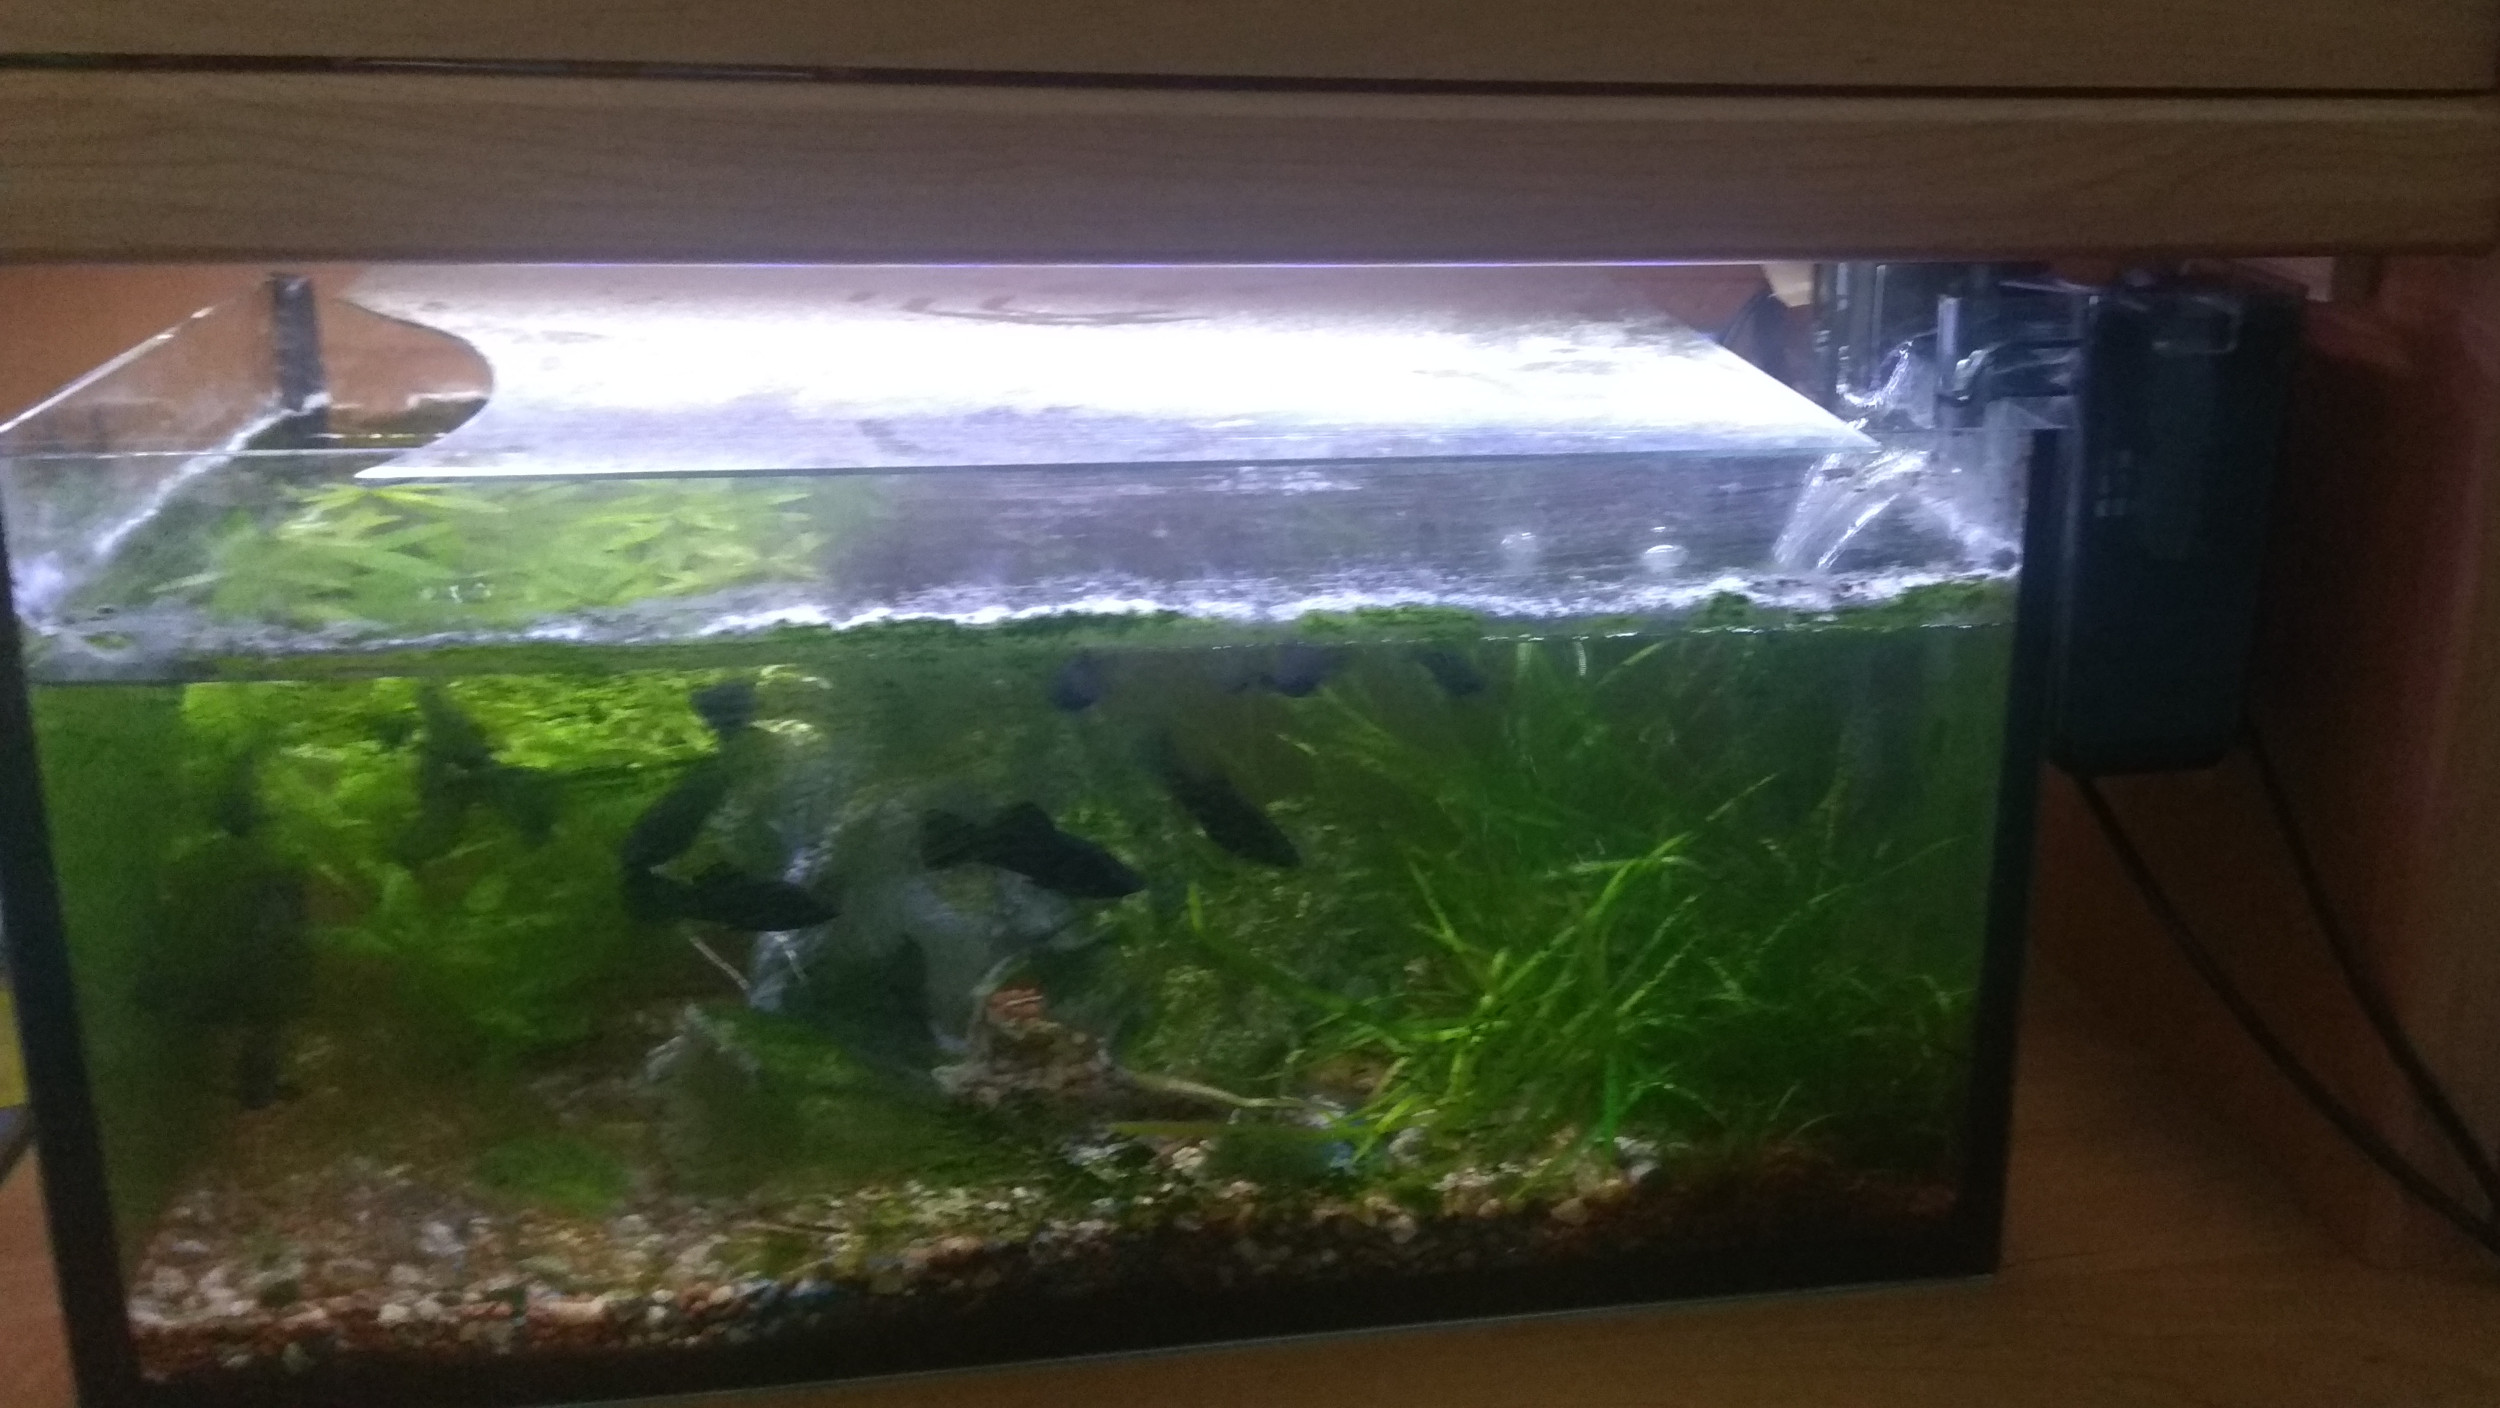
\includegraphics[width=0.8\textwidth]{akvarko.jpg}
		\caption{Naše akvárium, souhrnné foto.}
		\label{fig:akvarko}
	\end{figure}

	\begin{figure}[!h]
		\centering
		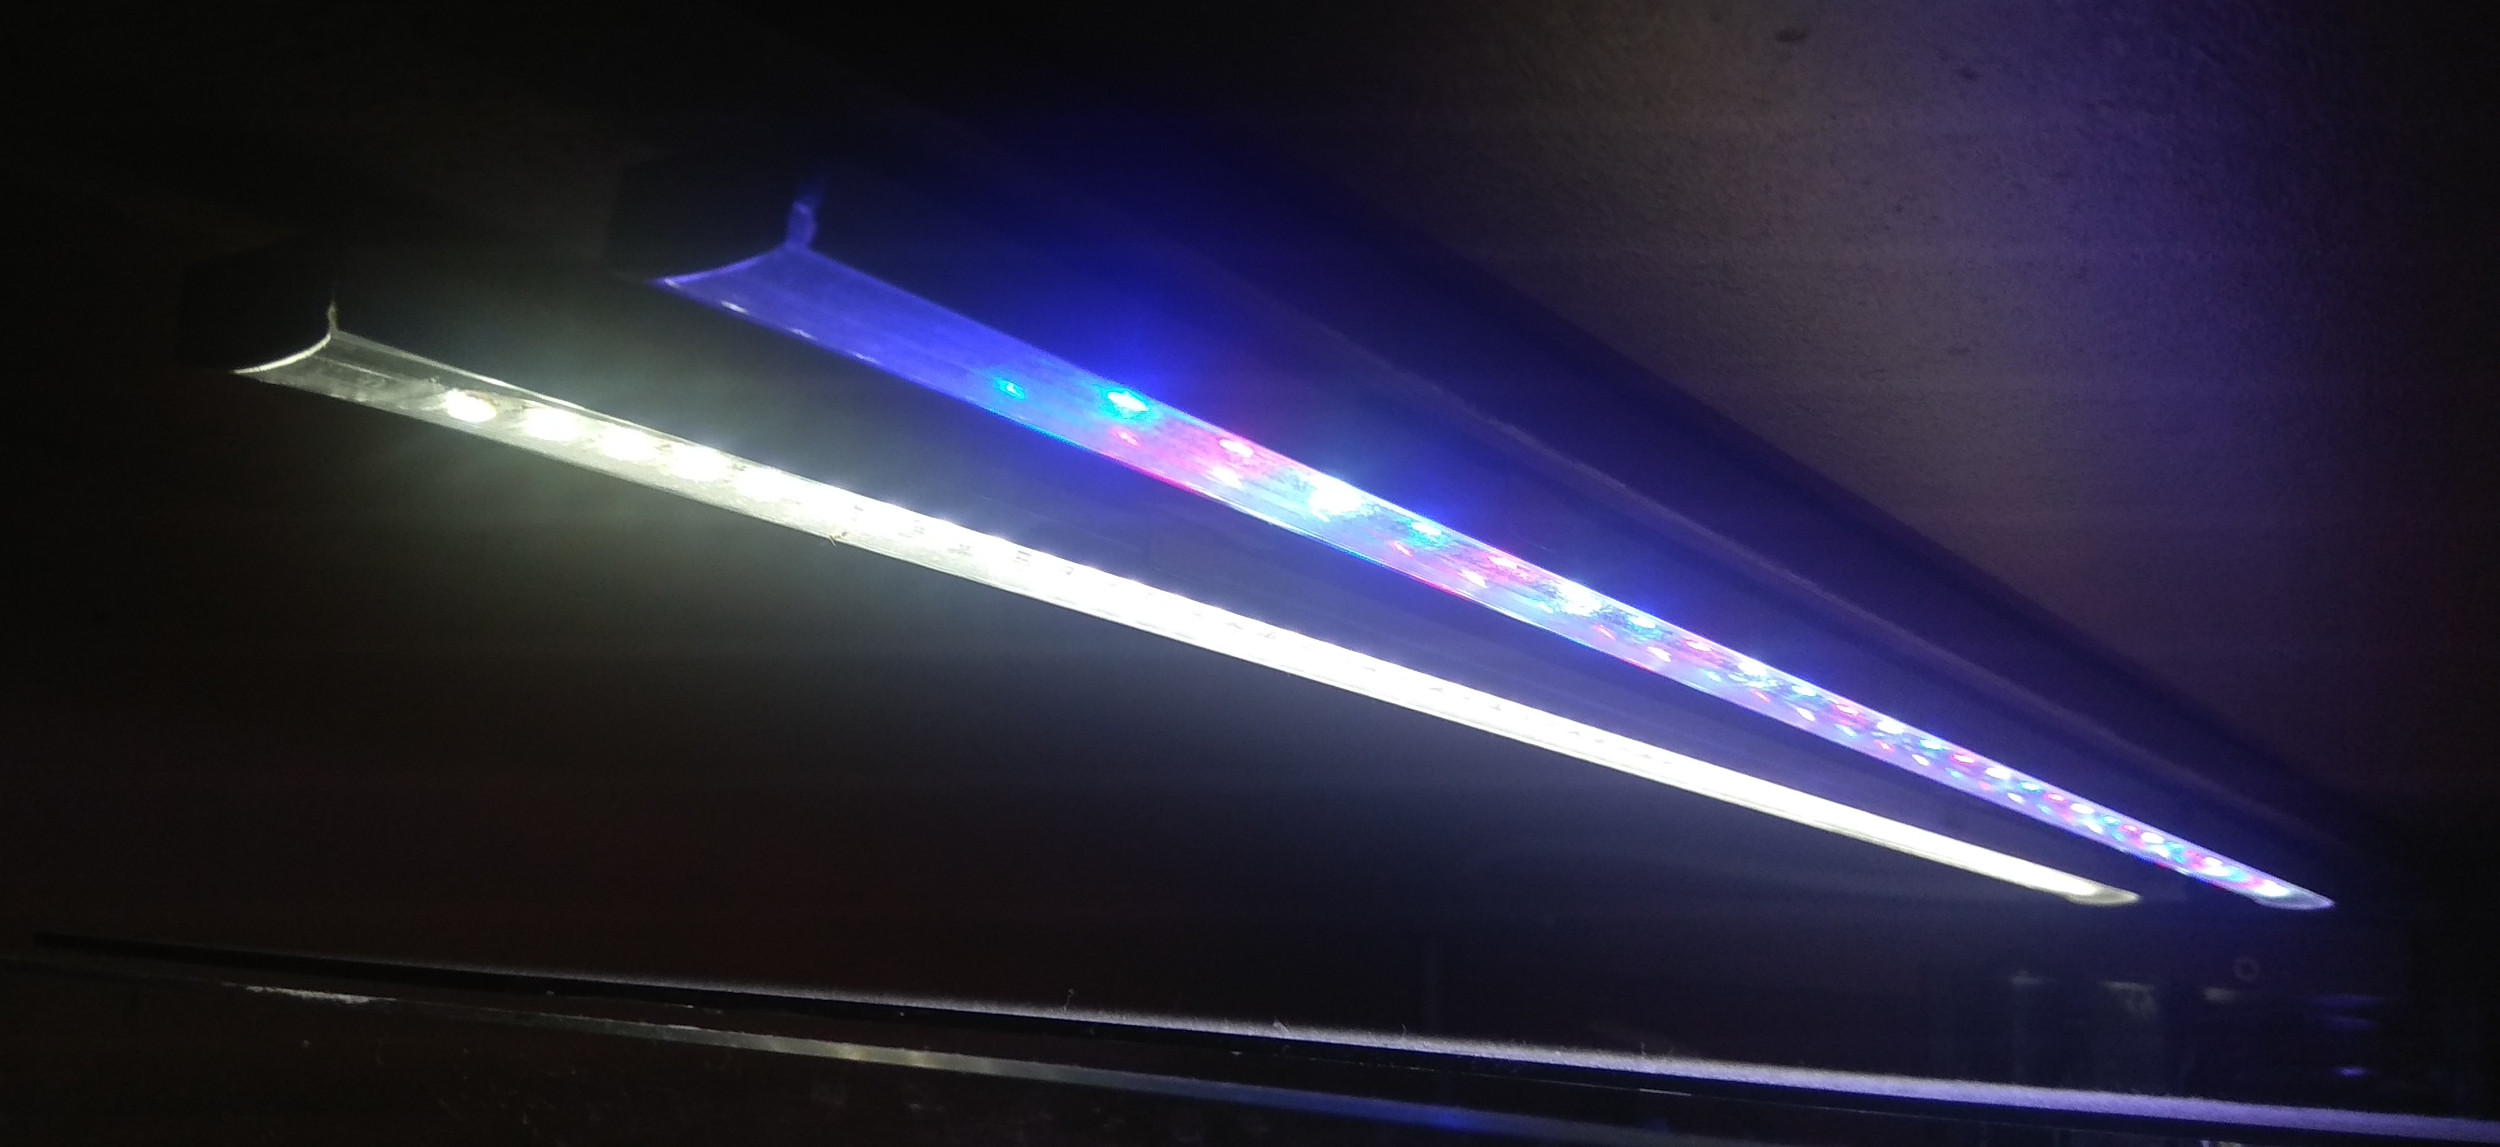
\includegraphics[width=0.8\textwidth]{svetla.jpg}
		\caption{Osvětlení formou dvou běžných LED pásků, ovládám každý zvlášť.}
		\label{fig:svetla}
	\end{figure}
	
	\begin{figure}[!h]
		\centering
		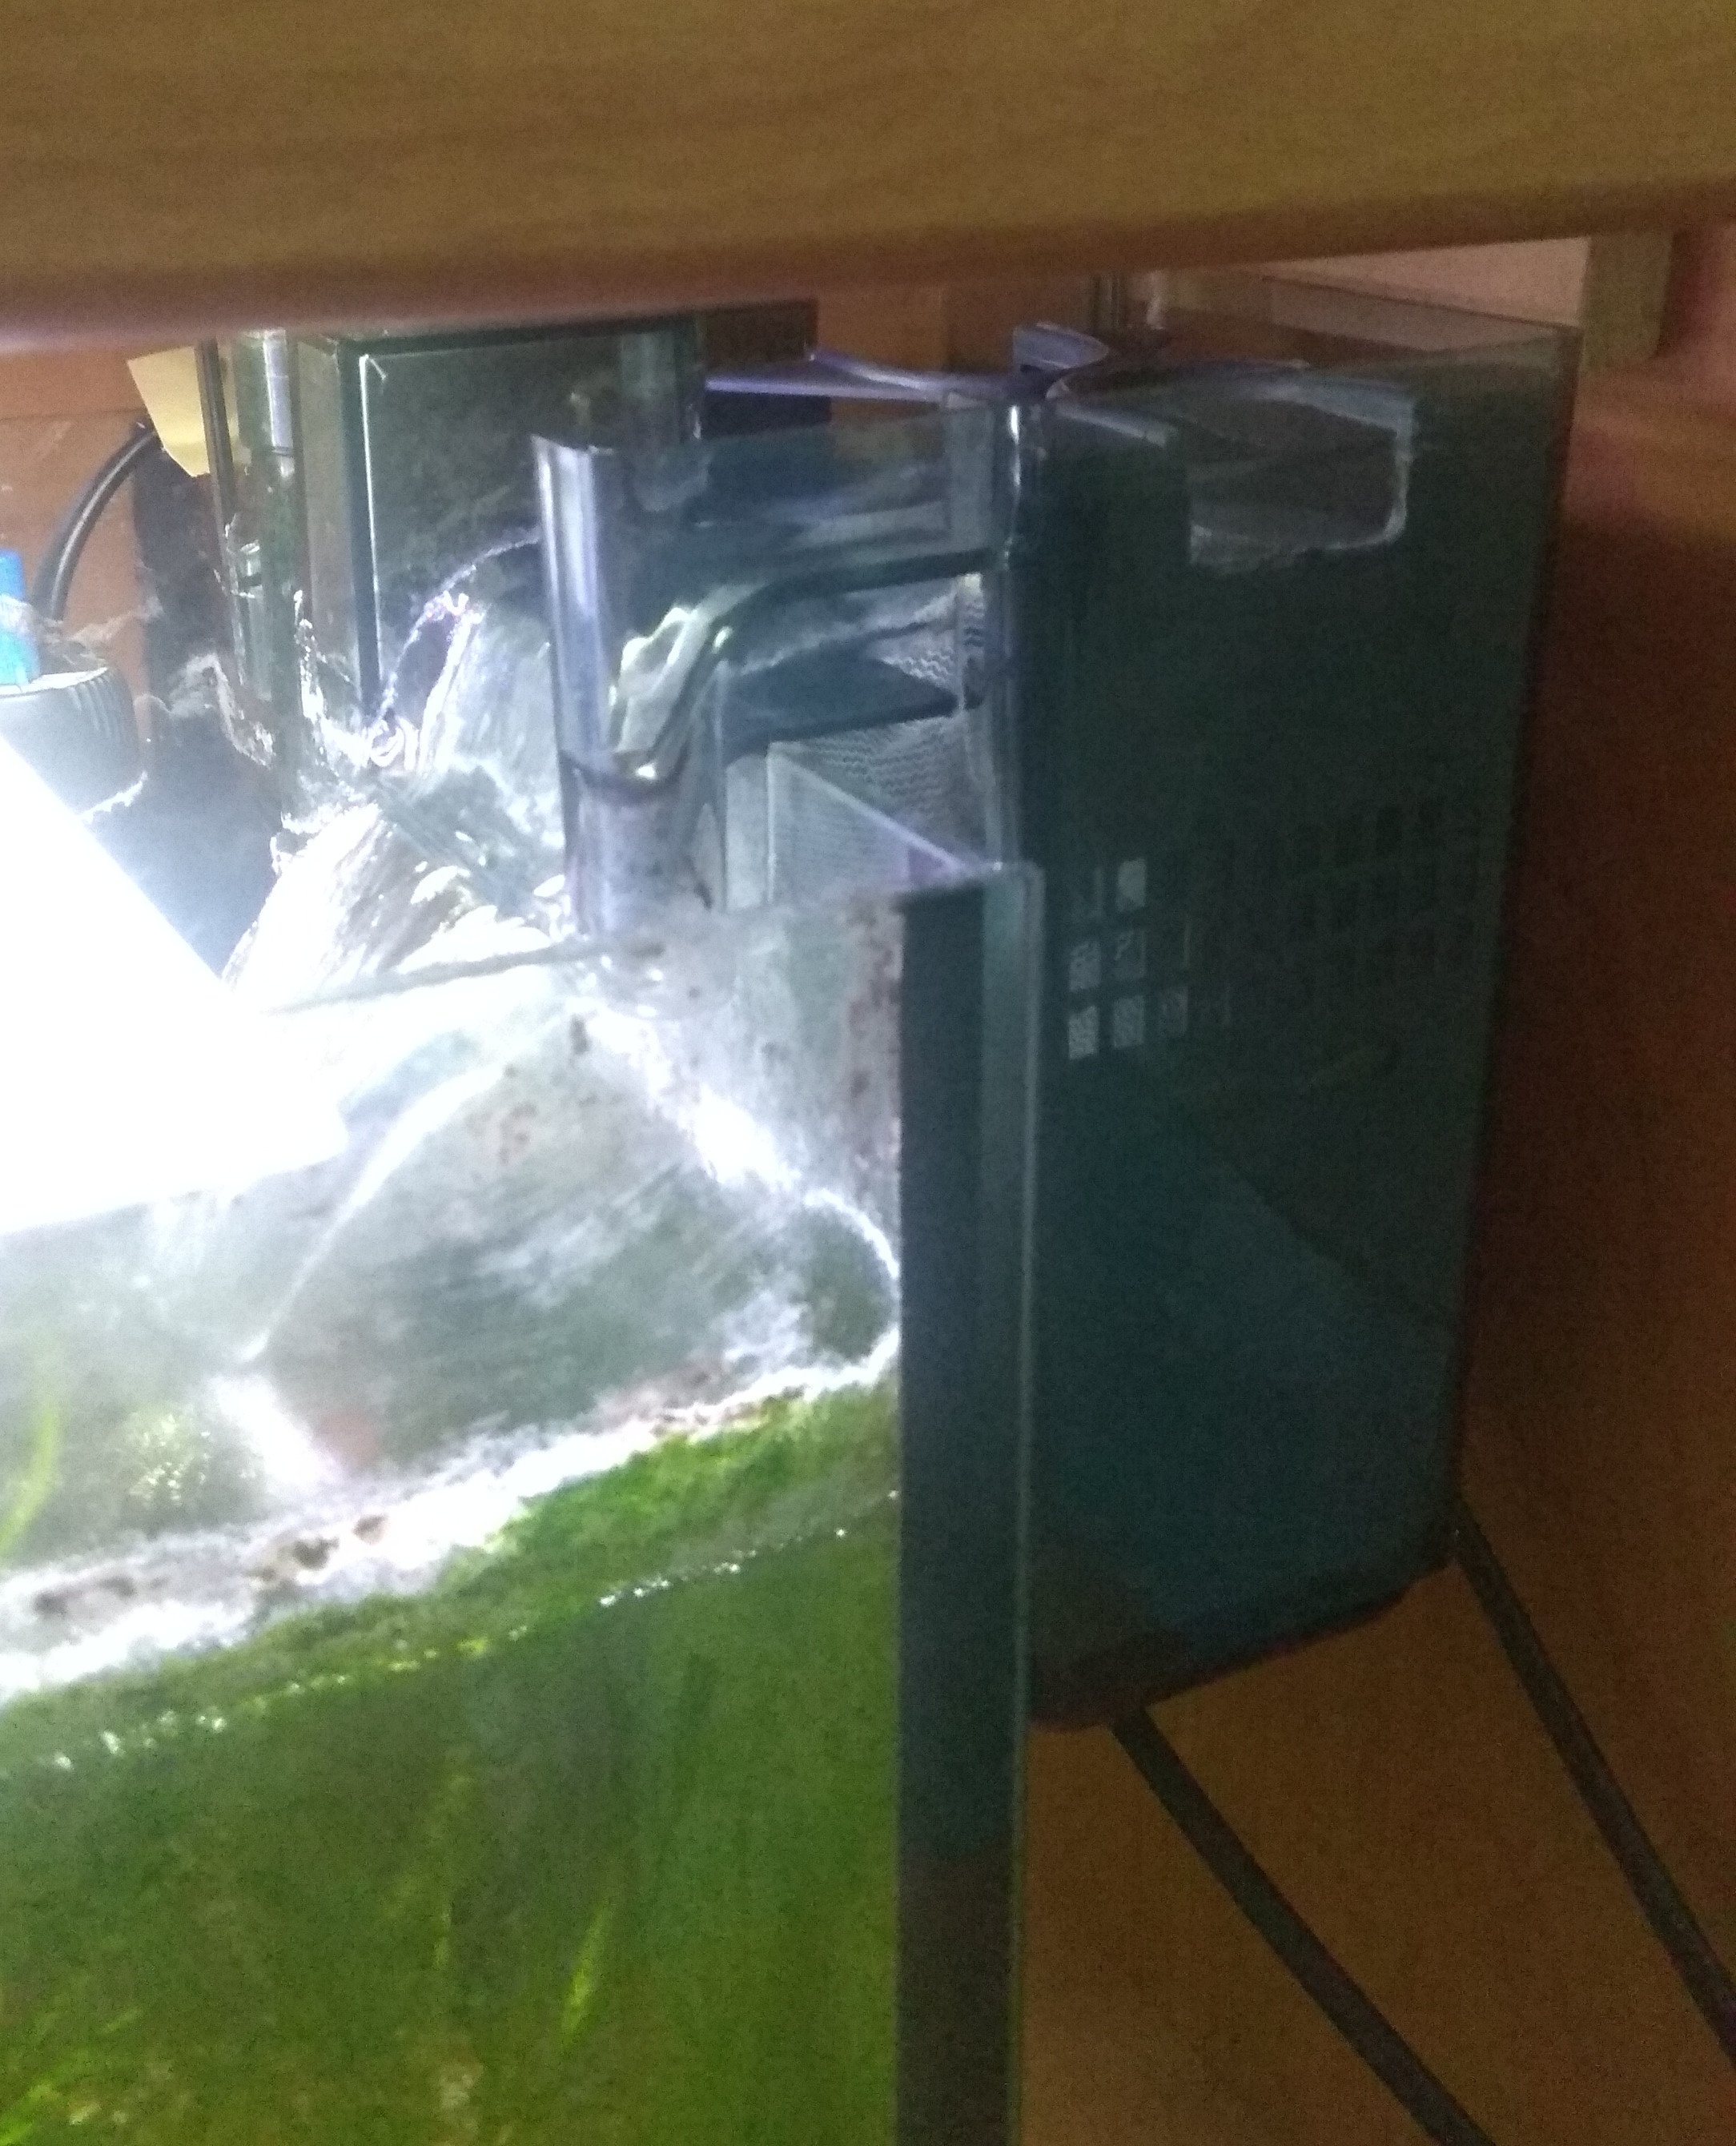
\includegraphics[width=0.6\textwidth]{filtr.jpg}
		\caption{Detail filtru.}
		\label{fig:filtr}
	\end{figure}

	\begin{figure}[!h]
		\centering
		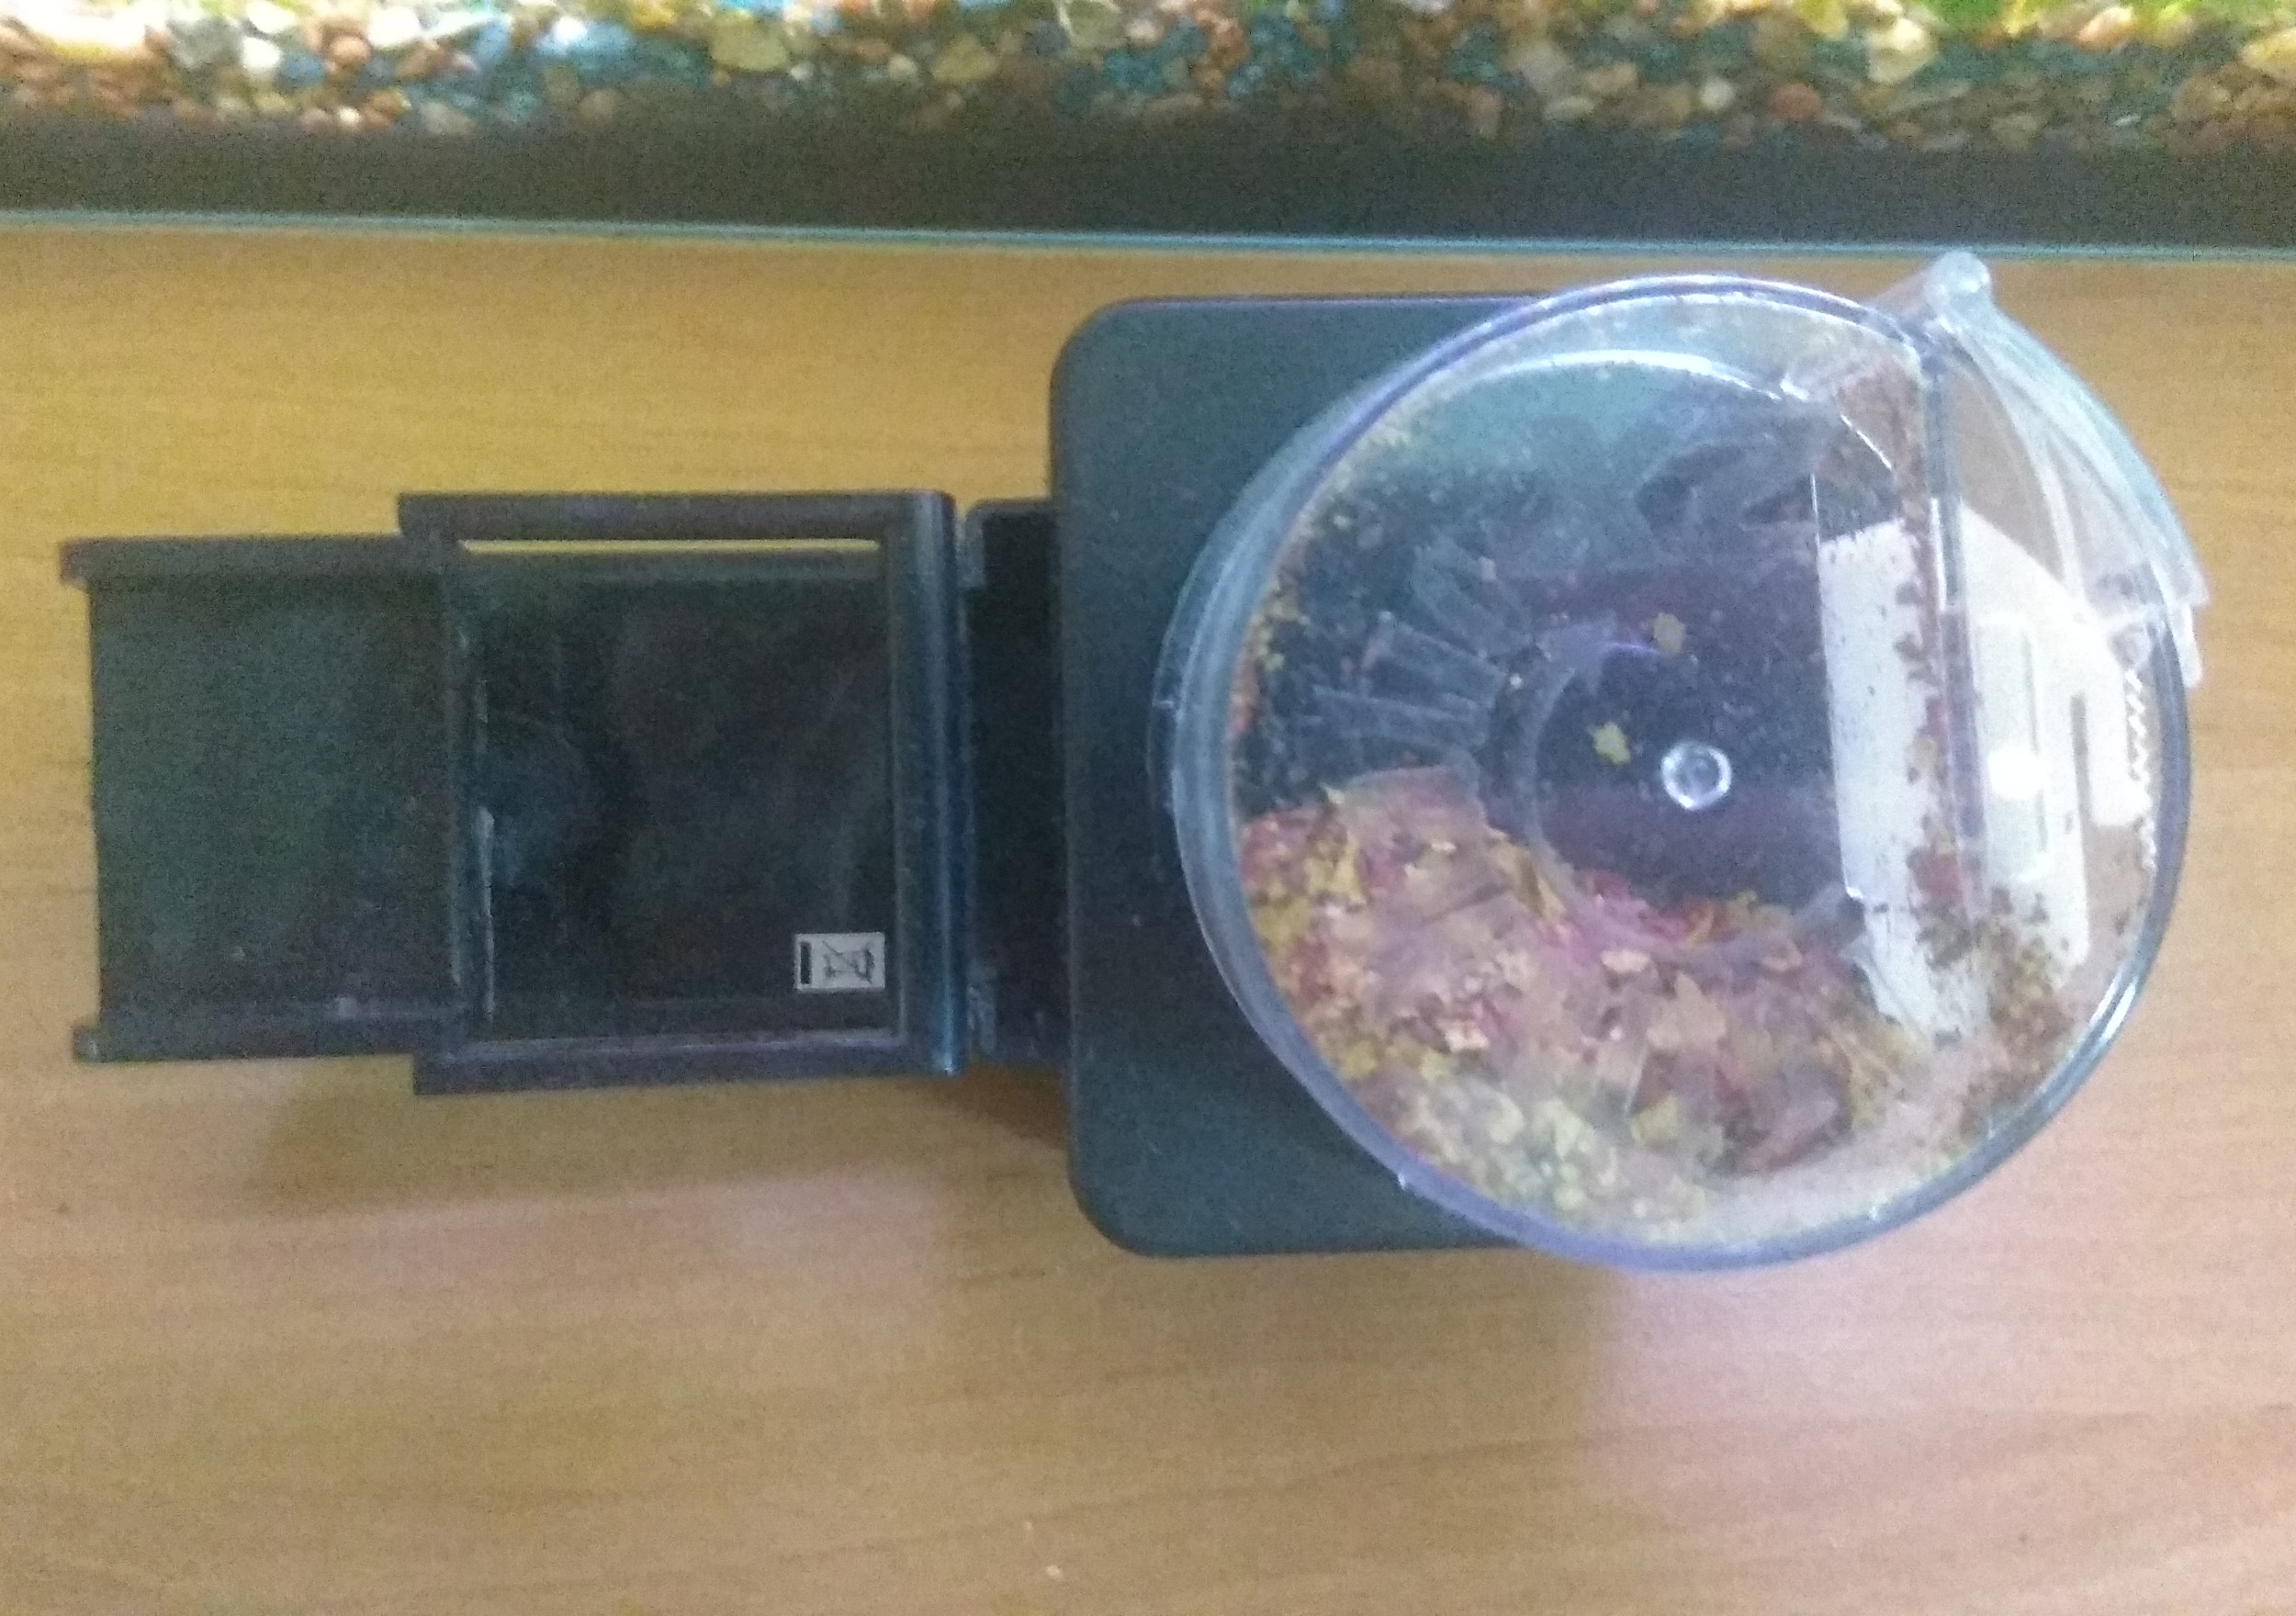
\includegraphics[width=0.8\textwidth]{krmitko.jpg}
		\caption{Automatické krmítko na baterie, rád bych nahradil vlastním řešením.}
		\label{fig:krmitko}
	\end{figure}


\clearpage
\section*{Popis verze Alpha :)}
	\begin{figure}[!h]
		\centering
		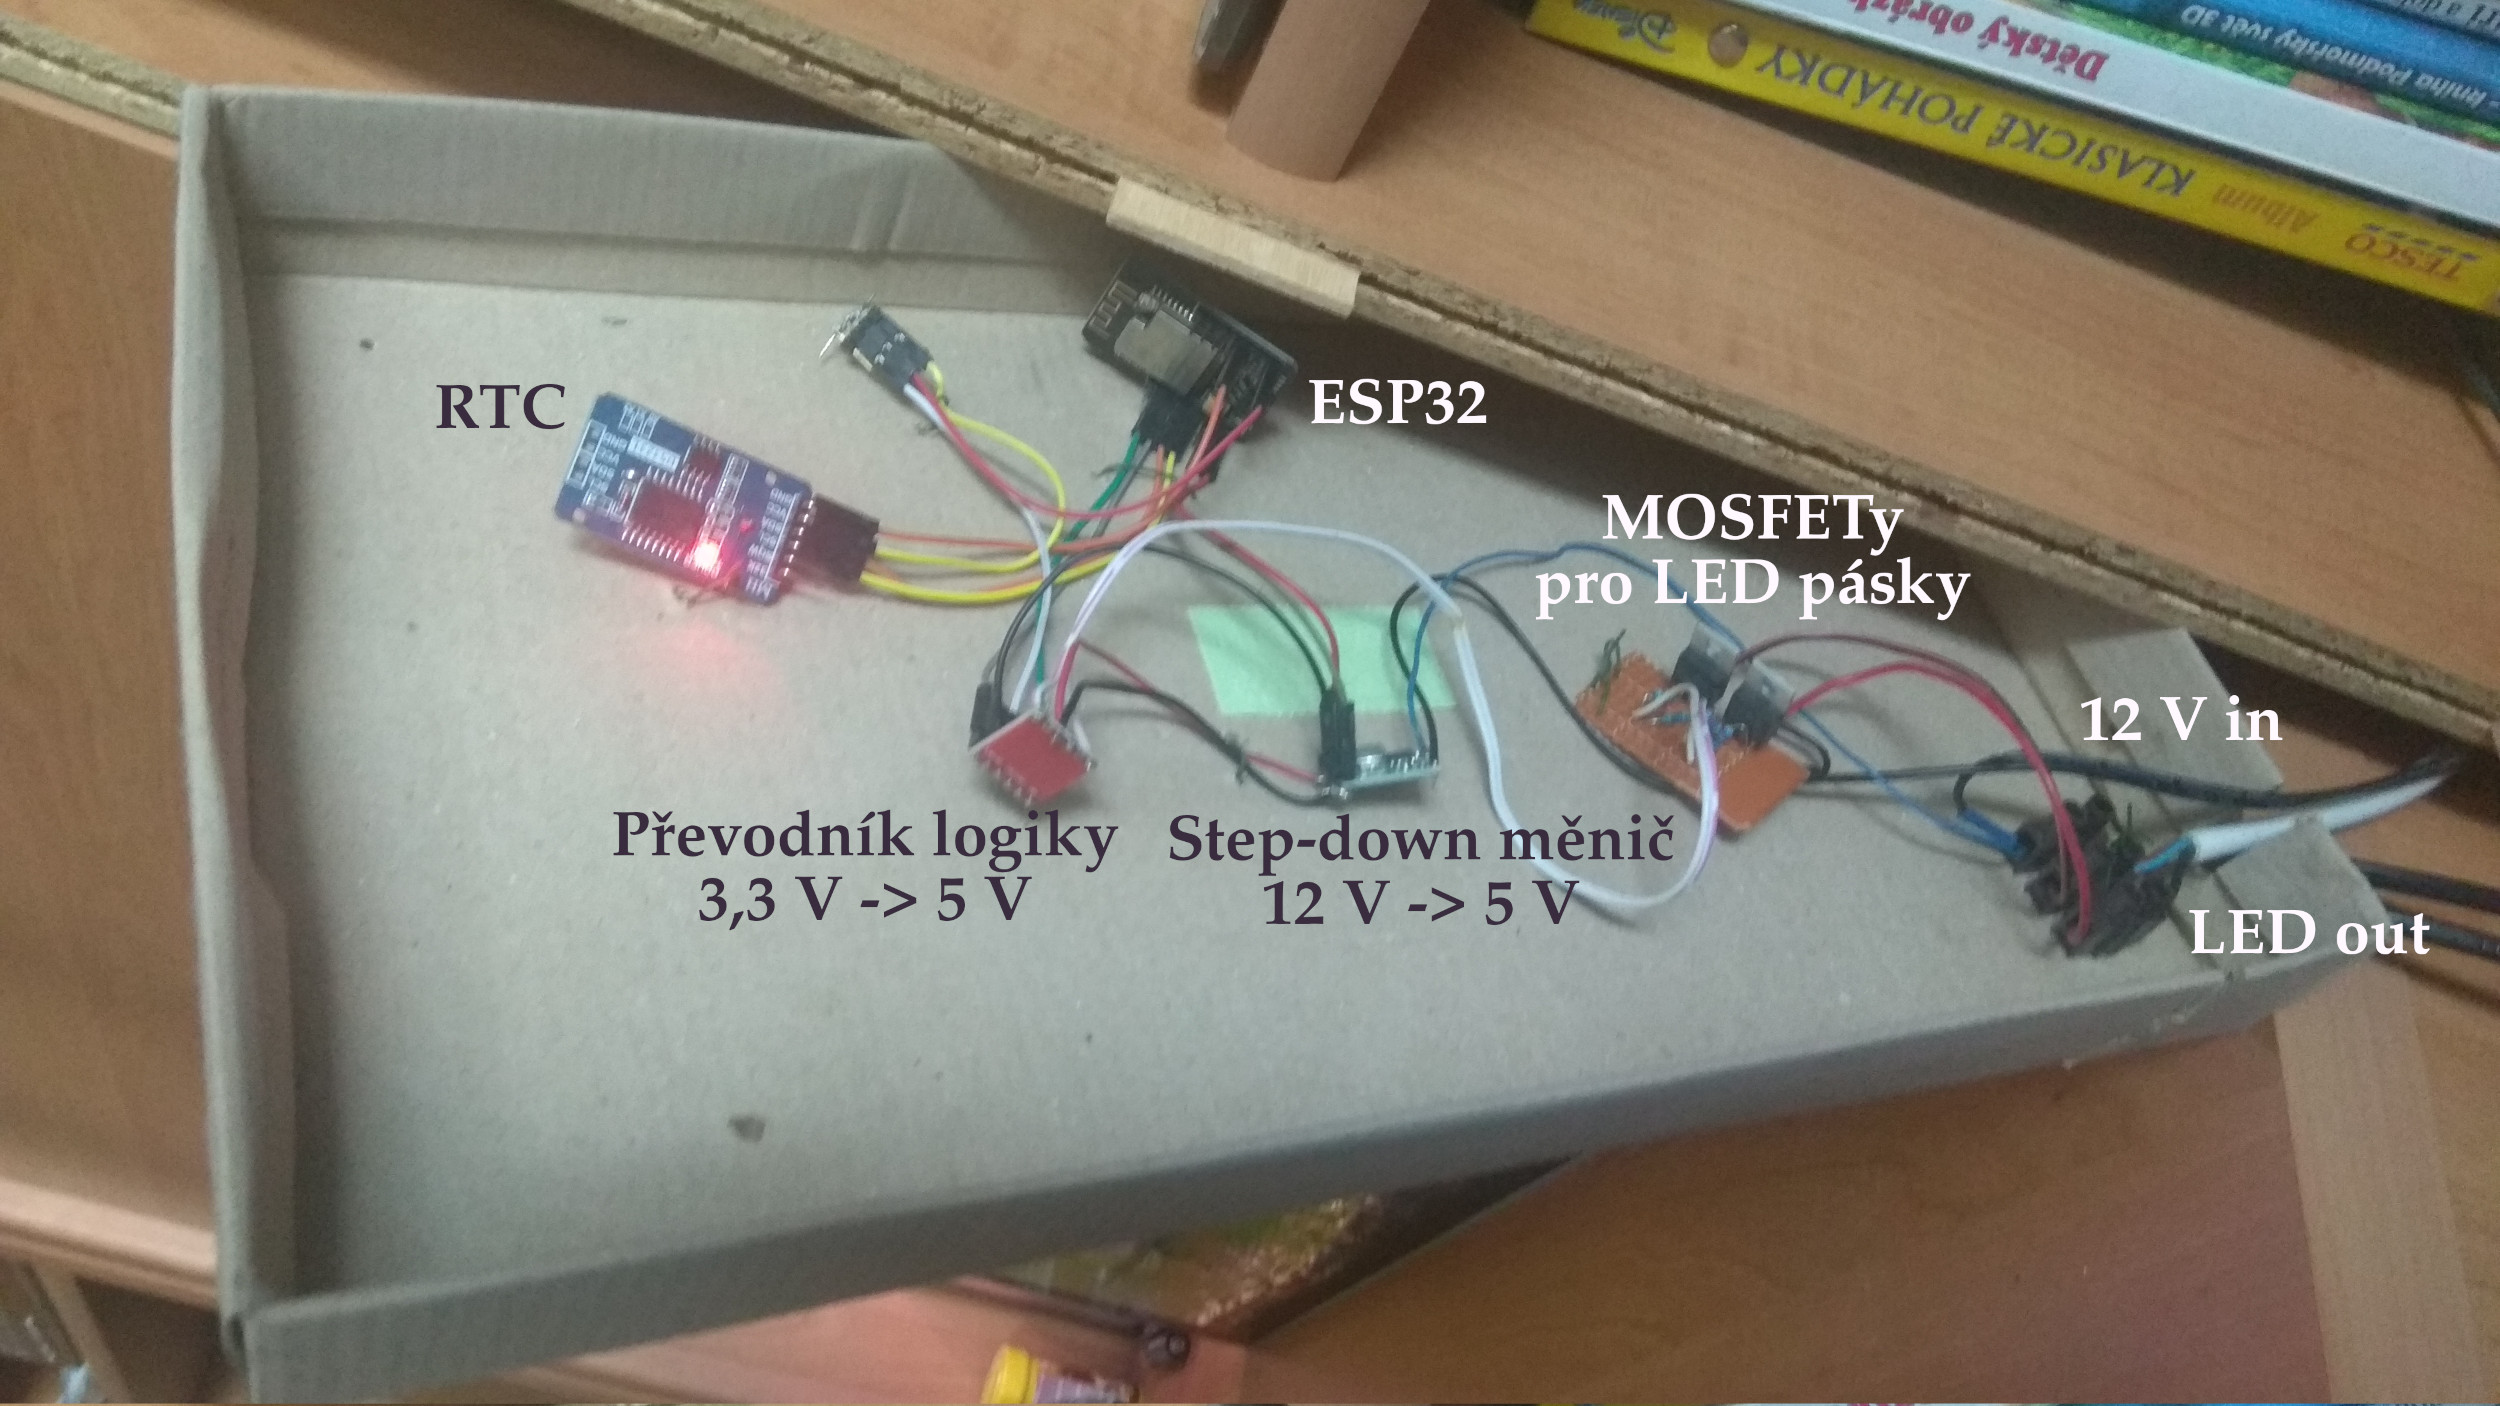
\includegraphics[width=0.9\textwidth]{moduly.jpg}
		\caption{moduly}
		\label{fig:moduly}
	\end{figure}
	Starší středoškolský projekt je vytvořený na úrovni modulů, je použit kontroler ESP32, na kterém běží webserver. Zařízení slouží pouze k ovládání světel, přes webovou stránku lze nastavit čas a rychlost rozsvícení a zhasnutí. 
	
	Kód je psán v Arduino frameworku, což byla v danou chvíli rozumná volba, ale teď bych se mu rád pokusil vyhnout. 
	Pro ovládání světel (LED pásky) jsem použil mosfet tranzistory řízené PWM pinem, také nebyly zvoleny vhodně, musel jsem použít předovník úrovně z \qty{3.3}{\volt} na \qty{5}{\volt}, aby bylo možné tranzistor plně otevřít.

	Za běžných podmínek zařízení funguje, ale například po výpadku elektřiny často končí v bootovací smyčce a je potřeba ručně zmáčknout reset, na stabilitu bych se tedy taky rád zaměřil.

\end{document}

